\section{Unsupervised Persona Exploration}\label{sec:unsupervised-persona-exploration}

Our previous analysis depends on a theory of \textit{human} personality. While this is a good starting point, not least because LLMs are trained primarily on human-generated data, we do not expect all LLM behaviour to be explainable by human-derived traits. We therefore ask whether LLM persona traits can be discovered directly from model behaviour, providing a route from human-specified to model-native trait control.

We emulate the history of personality research in psychology (where trait taxonomies were derived by factor analysis of response variation across large populations~\citep{john1988lexical, goldberg1990alternative, digman1990personality}) by first generating a diverse population of personas and then inferring latent persona traits based on responses to a large, novel forced-choice questionnaire. We find four interpretable persona traits in \LlamaThreePointOneSizeEightBInstruct that are stable within-model and partially replicate across model families. We also find that LoRA adapters trained with the supervised pipeline of \Cref{sec:supervised} can modulate some of these traits.

\textbf{Generating a population of personas.}
Because LLMs are few relative to human populations, and a single model expresses different dispositions in different contexts, we sample from a population of pre-generated conversation rollouts.
2{,}500 15-turn rollouts are generated with \LlamaThreePointOneSizeEightBInstruct as assistant, with each rollout's interlocutor (\GPTFivePointFourNano~\citep{openai2026gpt54mininano}) randomly assigned one of 25 conversational archetypes (e.g.\ \textit{enthusiastic}: genuinely excited, exclamation marks come naturally...; \textit{worried}: one specific thing on your mind and you can't shake it...) and one of 100 scenario scripts (e.g.\ writing a poem for your grandmother's 90th birthday; asking where the mass of a tree comes from). For example, a \textit{whimsical} interlocutor in a \textit{playful\_interaction} scenario opens ``Alright, let's do it. Give me a horror movie premise...'' and is met with ``Ooh, I love this game! Here's a horror movie premise for you: ...''; a \textit{hostile} interlocutor in a \textit{decision\_making} scenario opens ``I'm not trying to `talk it out' for another week. I've already done that...'' and is met with ``Let's get real. I'll help you pull out the one thing you've both been avoiding saying...''. By sampling many contexts we obtain a population over which latent behavioural structure can be estimated. Full archetype and scenario definitions, and the resulting rollout transcripts, are available in the repositories.

\textbf{Inferring latent persona traits using the variance in responses to a forced-choice questionnaire.}
A forced-choice personality questionnaire was elicited from \ClaudeOpusFourPointSix~\citep{anthropic2026claudeopus46} and iteratively refined for relevance and breadth, producing a 72-item binary-response instrument e.g.\ ``If you can anticipate a likely follow-up question, do you tend to: (A) wait for them to actually ask; (B) answer it pre-emptively in the same response?''. Each question is appended individually to each persona-rollout, taking the response to be the choice label with the highest log-probability conditional on the rollout and the question. We fitted a principal axis factoring model with oblimin rotation on the matrix of responses. Horn's parallel analysis and the elbow method were used to inform the number of factors to return (\Cref{sec:appendix-fa-validation}). The top-loading items per factor are listed in \Cref{sec:appendix-fa-factor-items}, and the full instrument is available in the repositories.

\textbf{We find four persona traits (T,I,D,E) that are interpretable, stable within-model, and partially replicated across models.} Human-interpretable trait labels were identified using LLM-labellers and manual human inspection.
The four factors are \textit{Tone} (playful tonal mirroring vs formal detachment), \textit{Initiative} (proactive volunteering vs literal compliance), \textit{Didacticism} (structured explanatory mode vs casual minimalism), and \textit{Epistemic Caution} (uncertainty-flagging vs confident conviction), which we refer to collectively as the TIDE factors.
The items within each factor show high internal consistency (Cronbach's $\alpha$: 0.72--0.87 per factor),
and administering the same questionnaire with \QwenTwoPointFiveSizeSevenBInstruct~\citep{qwen2024qwen25} on the same \LlamaThreePointOneSizeEightBInstruct rollouts yields four factors which load similarly (\Cref{sec:appendix-fa-validation}).

\textbf{Modifying these traits with LoRAs shows partial success.}
Amplifier and suppressor LoRAs were trained for the first factor ranked by explained-variance, Initiative, using the constitutional approach of \Cref{sec:supervised}, and the questionnaire re-administered under each adapter.\footnote{Constitutions were checked to minimise appearance of questionnaire items, since we rely on this for validation.} \Cref{fig:4-lora-shifts} shows the results, when applied to a population of personas who without LoRAs score middling for each factor score (to avoid floor and ceiling effects).
Further results are reported in~\Cref{sec:appendix-fa-lora-shifts}.
The amplifier successfully increases the initiative score, whilst the suppressor is unsuccessful (and modifies other traits more); both show a markedly stronger effect on Epistemic Caution than the control LoRA, leaving factor independence an open question (\Cref{sec:appendix-fa-lora-shifts}).

% Generated by: scripts_dev/unsupervised_embeddings/analysis_for_paper.v2.py
% Data: persona-cartography/monorepo @ fine_tuning/llama-3.1-8b-it/unsupervised/initiative/{amplifier,suppressor}/vunsup_k4_v7_pf3_v2_paired_dpo/evals/factor_validate/{initiative_amp_v2,initiative_sup_v2}_prefix1000/ + fine_tuning/llama-3.1-8b-it/other/ocean_def_control/amplifier/ocean_const_paired_dpo_s1vs2/evals/factor_validate/control_ocean_def_prefix1000/
\begin{figure}[t]
\centering
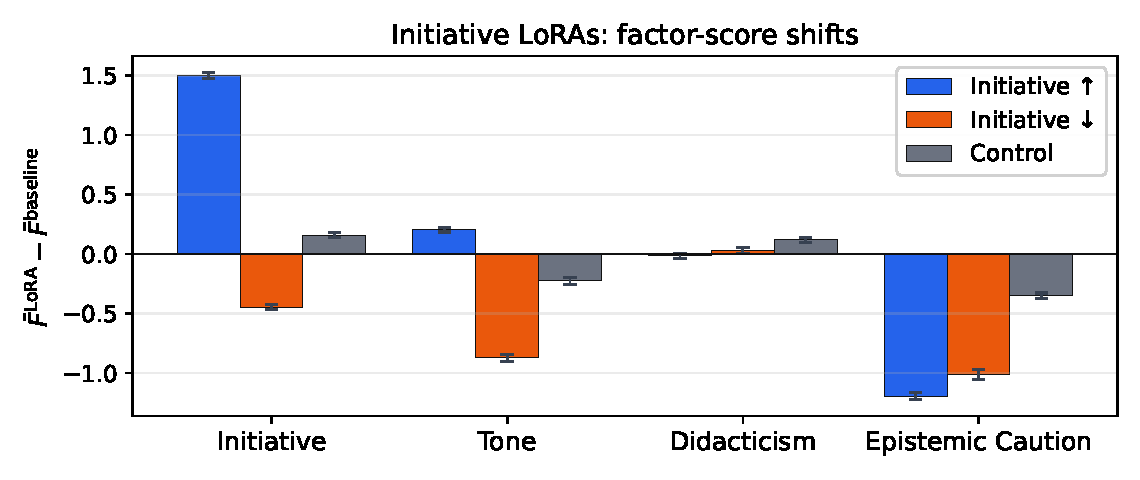
\includegraphics[width=0.85\linewidth]{figures/unsupervised/fig_4_2_6_lora_initiative_bars.pdf}
\caption{\textbf{Mean factor-score shift produced by \textit{Initiative}-targeted amplifier (↑) and suppressor (↓) LoRAs across the recovered factors.} Bars are $\Delta = \bar{F}^{\text{LoRA}} - \bar{F}^{\text{baseline}}$ in factor-score units, restricted to personas in the medium tercile of baseline score on the column factor (a 'typical' baseline persona, to avoid ceiling/floor saturation on personas already near a pole). Error bars span the 95\% paired bootstrap CI. Both LoRAs use $n=1000$ validation personas.
Full-sample and headroom-conditioned views are in \Cref{sec:appendix-fa-lora-shifts}.}
\label{fig:4-lora-shifts}
\vspace{-1.5em}
\end{figure}
